%%%%%%%%%%%%%%%%%%%%%%%%%%%%%%%%%%%%%%%%%
% Wenneker Article
% LaTeX Template
% Version 2.0 (28/2/17)
%
% This template was downloaded from:
% http://www.LaTeXTemplates.com
%
% Authors:
% Vel (vel@LaTeXTemplates.com)
% Frits Wenneker
%
% License:
% CC BY-NC-SA 3.0 (http://creativecommons.org/licenses/by-nc-sa/3.0/)
%
%%%%%%%%%%%%%%%%%%%%%%%%%%%%%%%%%%%%%%%%%

%----------------------------------------------------------------------------------------
%	PACKAGES AND OTHER DOCUMENT CONFIGURATIONS
%----------------------------------------------------------------------------------------

%\documentclass[10pt, a4paper, twocolumn]{article} % 10pt font size (11 and 12 also possible), A4 paper (letterpaper for US letter) and two column layout (remove for one column)
\documentclass[10pt, a4paper, twocolumn]{ctexart}
\input{structure.tex} % Specifies the document structure and loads requires packages

%----------------------------------------------------------------------------------------
%	ARTICLE INFORMATION
%----------------------------------------------------------------------------------------



% Example of a one line author/institution relationship
%\author{\newauthor{John Marston} \newinstitution{Universidad Nacional Autónoma de México, Mexico City, Mexico}}

%\date{\today} % Add a date here if you would like one to appear underneath the title block, use \today for the current date, leave empty for no date
\date{}
%----------------------------------------------------------------------------------------
\setlength{\textfloatsep}{5pt}
\begin{document}
	\title{暗恋经历与被暗恋经历调查报告} % The article title

	\author{
		\authorstyle{ 李侑性1 李旭坤2 杨庆龙2} % Authors
		\newline\newline % Space before institutions
		\textsuperscript{1}\institution{中国语言文学系}\\ % Institution 1
		\textsuperscript{2}\institution{信息科学技术学院}}
	}
\maketitle % Print the title

\thispagestyle{firstpage} % Apply the page style for the first page (no headers and footers)

%----------------------------------------------------------------------------------------
%	ABSTRACT
%----------------------------------------------------------------------------------------

\lettrineabstract{本文通过对一定数量的暗恋经历与被暗恋经历的统计学分析,检验了一些关于暗恋的常见刻板印象,并试图通过这些分析给暗恋中的单身人士一些建议,帮助他们更好地表达自己的心意。}
\\
%----------------------------------------------------------------------------------------
%	ARTICLE CONTENTS
%----------------------------------------------------------------------------------------
\section{引言}
暗恋几乎是每个人都会经历的情感阶段,然而实际上能走到一起的人却很少。毕竟对别人有好感很容易,但向别人表达自己的好感却很难,而自己的好感能被接受就更难了。因此,我们试图通过分析各种各样的暗恋经历和被暗恋经历,给处在暗恋阶段中的人一些指导,帮助他们早日脱单。\\
\section{样本描述}
在本次调查中,我们从北京大学在校学生中收集了学院、性别和入学时间等基本信息,并简单地从时间,环境,告白方式等方面调查他们的暗恋经历与被暗恋经历。\\
\subsection{基本信息}
我们共收集了270份有效问卷,涵盖了所有本科年级与学院,其中又以信息科学技术学院的2018级本科生占绝大部分。由于外貌也是个人吸引力的一大重要因素,所以我们也想将其收入暗恋经历的影响因素之一,但由于无法很好地在问卷中量化一个人的长相,所以我们选用BMI指数作为外貌维度的主要指标。此外,我们将人群简单分为是否有过暗恋与是否有过被暗恋经历共四类人群。对于有过暗恋经历或被暗恋经历的被试,我们又从时间节点,环境影响以及告白等因素上进行更为细致的调查。\\\\\\
\subsection{暗恋经历与被暗恋经历信息}
\subsubsection{时间因素}
在一般情况下暗恋应该经历认识暗恋对象,对暗恋对象萌生好感两个必要的时间节点,以及可能经历的告白节点。考虑到被测试人员对时间的记忆能力等因素,我们选择使用XX年级YY月的形式调查这些时间节点的时间,并通过将一年级入学年的1月定义为0月来实现时间维度上的量化调查。
\begin{figure}[htbp]
	\subfigure[性别比例图] {
	\centering
	\label{c0}
	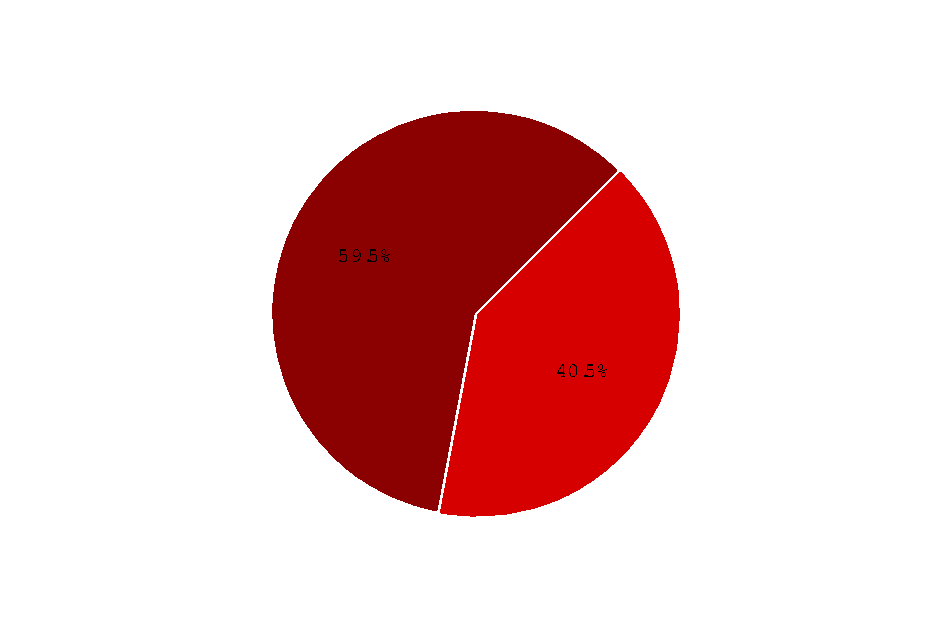
\includegraphics[width = 0.8\linewidth]{c0.eps}
	}
	\quad
	\subfigure[学院比例图] {
	\centering
	\label{c1}
	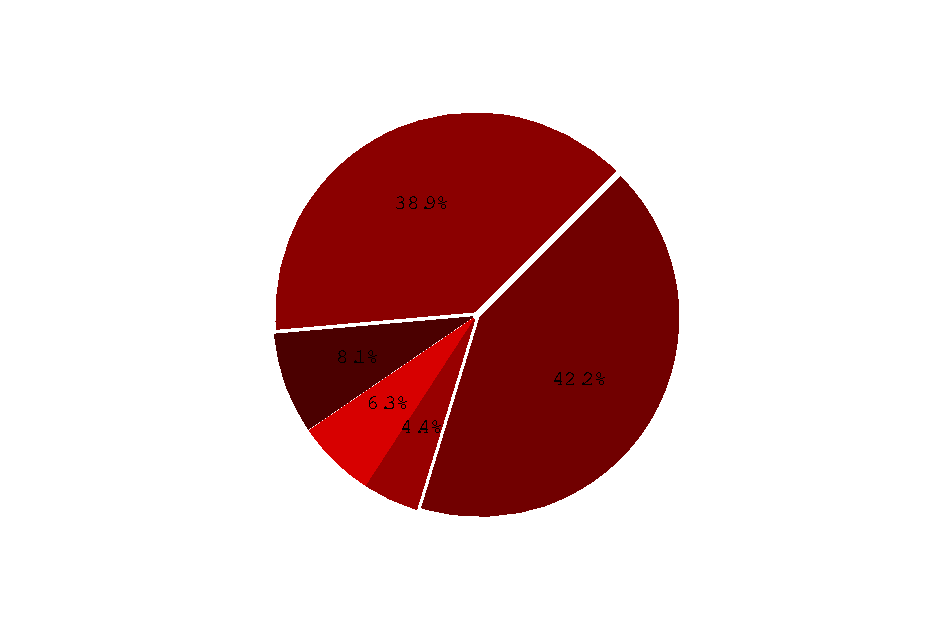
\includegraphics[width = 0.8\linewidth]{c1.eps}
	}
	\caption{被试基本信息图} % Figure caption
\end{figure}

从我们的统计数据\ref{c5}中可以看到,由于我们的被试人员主要来自于2018级本科生,导致大部分被试人员是在初中与高中入学时认识暗恋对象的,而在大学认识相对较少。\\
\indent 而暗恋开始时间则相对比较分散,并没有出现特别集中分布的趋势,如图\ref{c18}。并不是每一段暗恋都会以告白结束,其具体比例如图\ref{c8}。对于告白的那部分人,他们的告白时间点集中于高三,高二与大一,与大家一般认为的高三毕业后的告白浪潮相符。对于被暗恋方也有着相类似的结论,而且比较暗恋开始时间与意识到被暗恋的时间我们可以发现,被暗恋方在暗恋方暗恋前就已经有所察觉,这可以在一定程度上说明暗恋方表现出自己好感的迹象远比自己想象中的明显。\\

\begin{figure}[htbp]
	\subfigure[认识时间分布图] {
	\centering
	\label{c5}
	\includegraphics[width = 0.8\linewidth]{c5.eps}
	}
	\quad
	\subfigure[暗恋开始时间分布图] {
	\centering
	\label{c18}
	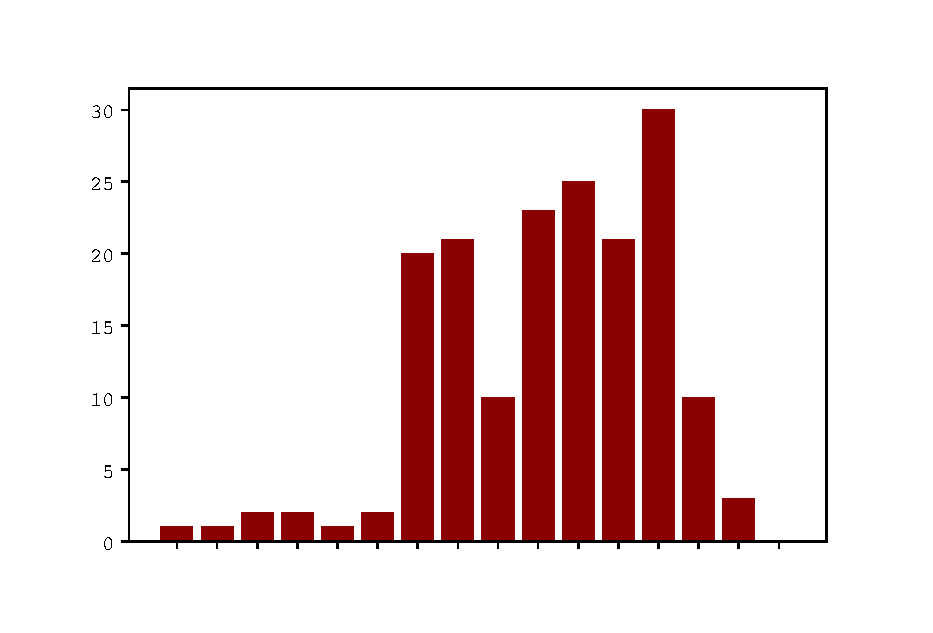
\includegraphics[width = 0.8\linewidth]{c18.eps}
	}
	\quad
	\subfigure[告白时间分布图] {
	\centering
	\label{c8}
	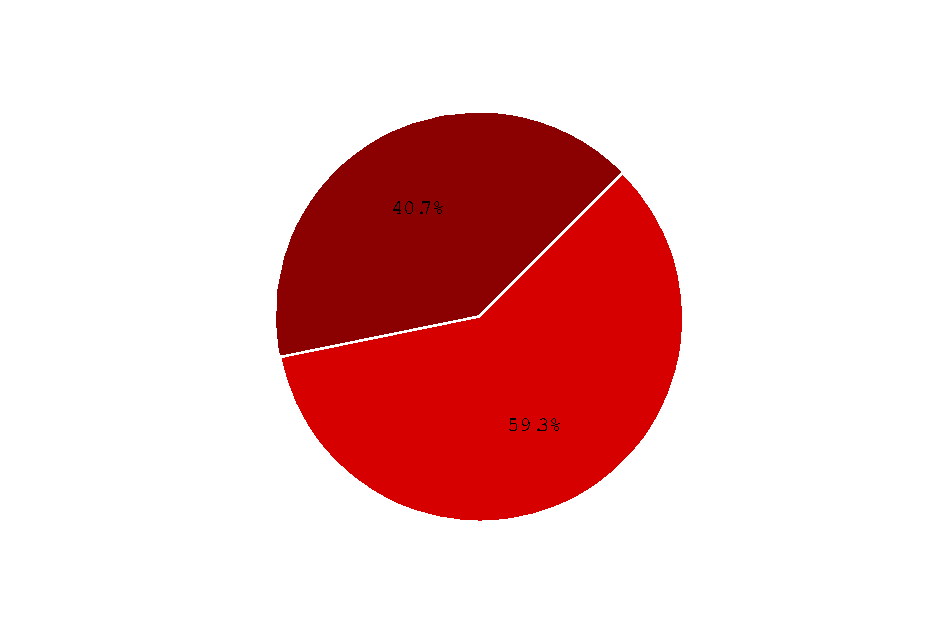
\includegraphics[width = 0.8\linewidth]{c8.eps}
	}
	\caption{暗恋经历统计图} % Figure caption
\end{figure}


\begin{figure}[htbp]
	\subfigure[认识时间分布图] {
	\centering
	\label{c19}
	\includegraphics[width = 0.8\linewidth]{c19.eps}
	}
	\quad
	\subfigure[发现被暗恋时间分布图] {
	\centering
	\label{c20}
	\includegraphics[width = 0.8\linewidth]{c20.eps}
	}
	\quad
	\subfigure[被告白时间分布图] {
	\centering
	\label{c15}
	\includegraphics[width = 0.8\linewidth]{c15.eps}
	}
	\caption{被暗恋经历统计图} % Figure caption
\end{figure}
\subsubsection{环境因素}

由于我们的被试人员暗恋发生时都处在学生阶段,而学生阶段的暗恋又不可避免地会出现同学起哄的情况。所以我们选择被试人员对同学的评分作为对环境因素测量的依据。从图\ref{c7}中可以看到评分有两个峰,0分处的峰表示被试人员认为朋友在全程添乱,没有给予任何帮助;而5分处的峰则表示朋友的表现好坏掺半,总体来说,很少有被试人员并认为身边的朋友能够帮助自己脱单。而对于被暗恋方来说,也认为朋友在整个过程除了没用就算添乱。\\
\begin{figure}[htbp]
	\subfigure[暗恋方评分] {
	\centering
	\label{c7}
	\includegraphics[width = 0.8\linewidth]{c7.eps}
	}
	\quad
	\subfigure[被暗恋方评分] {
	\centering
	\label{c13}
	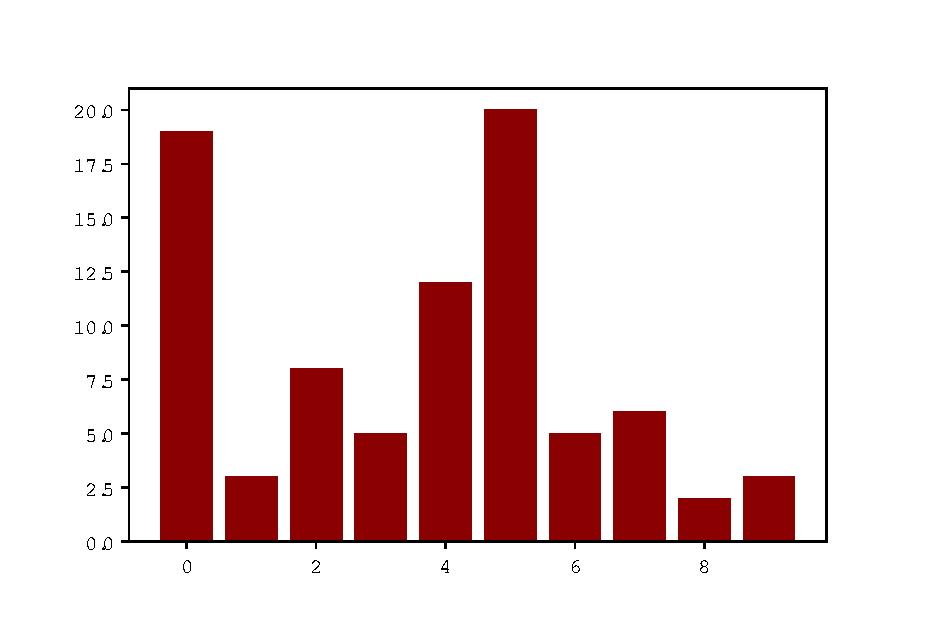
\includegraphics[width = 0.8\linewidth]{c13.eps}
	}
	\caption{朋友评分统计图} % Figure caption
\end{figure}
\subsubsection{告白表达因素}

告白方式也是决定一段暗恋是否成功的重要因素之一,所以我们对被试人员的告白方式进行了统计,如图\ref{c11}。从图中可以看到,得益于即时通讯工具的发展,大部分人选择的是在线文字聊天的方式进行告白。面对面告白与写情书的比例次之,且两者差别不大,但它们都远远不及使用在线文字告白的人数。而对于被暗恋方,也能得到相同的结论。\\
\begin{figure}[htbp]
	\subfigure[暗恋方评分] {
	\centering
	\label{c11}
	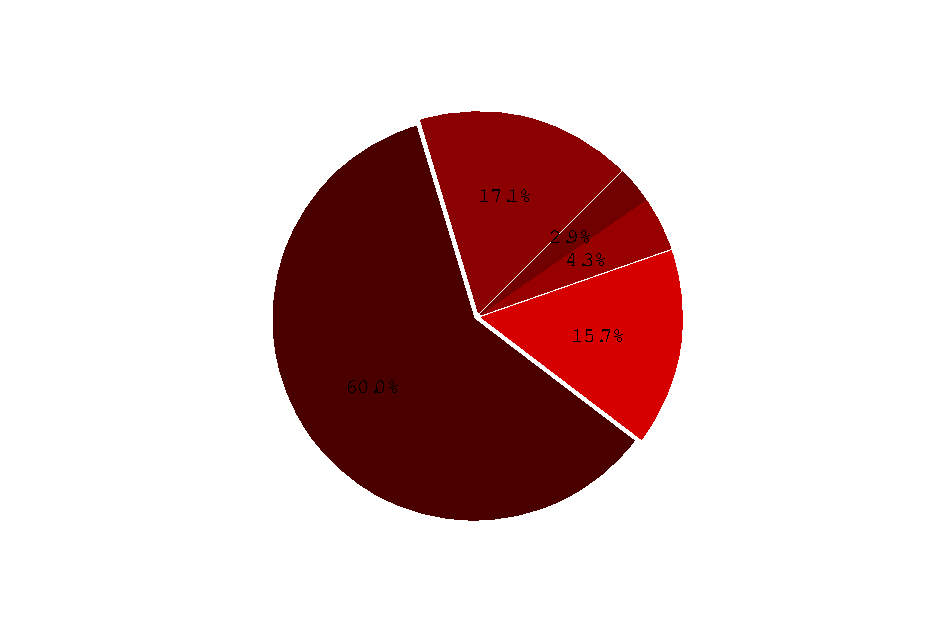
\includegraphics[width = 0.8\linewidth]{c11.eps}
	}
	\quad
	\subfigure[被暗恋方评分] {
	\centering
	\label{c17}
	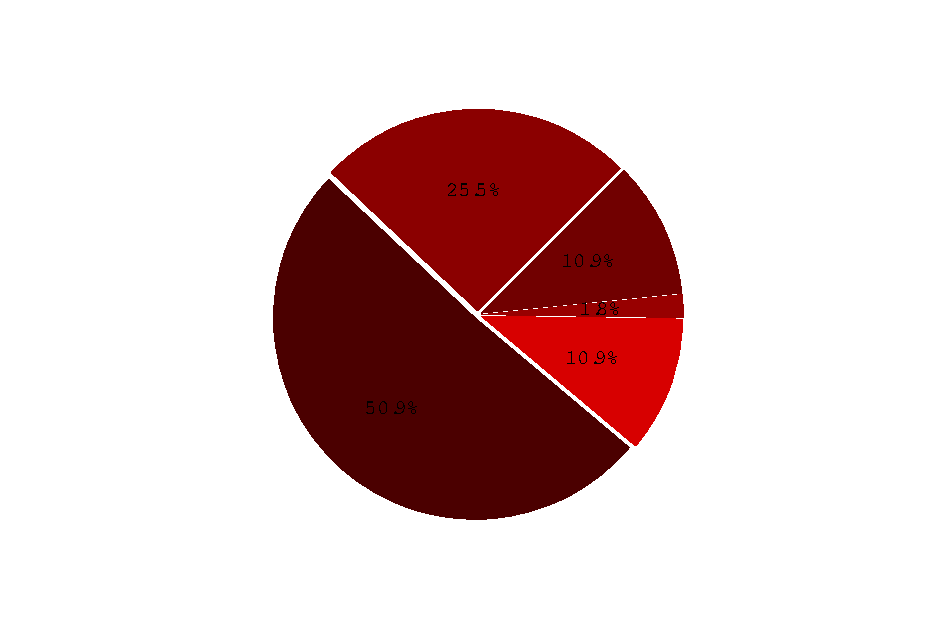
\includegraphics[width = 0.8\linewidth]{c17.eps}
	}
	\caption{告白方式统计图} % Figure caption
\end{figure}
\indent 除了告白方式,告白时的表现也是决定告白是否成功的重要的因素之一。但是,直接让被试给告白时的自己打分显然不可靠。所以,我们通过比较被试对于自己告白成功的把握以及告白后的结果进行比较,可以得到统计图如下。\\

\begin{figure}[htbp]
	\lcaption{告白把握与结果统计图}
	\centering
	\label{c100}
	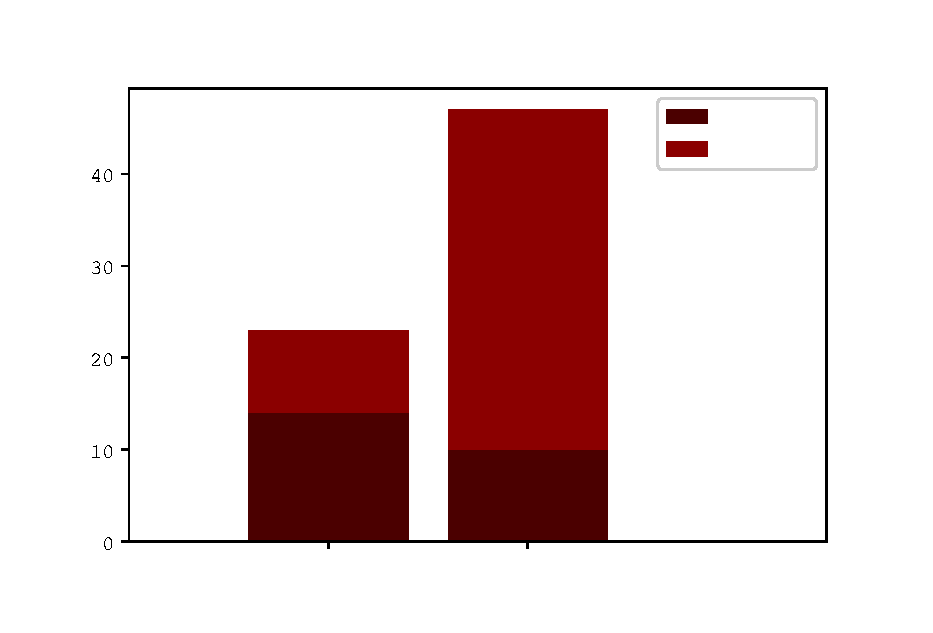
\includegraphics[width = 0.8\linewidth]{c12.eps}
\end{figure}

\section{卡方相关性检验}
\subsection{性别与暗恋类型}
\\\\\\\\\\在性别与暗恋类型中发现,其实两者之间没有明显的相关性。卡方检验中实际距离大致为22.07,而这数据与6个项目相比小于它们的理论距离。爱是人类生来具有的天然性感情。相似性和相互依恋等其产生因素并不局限于性别。因为爱本身的核心特质在于普遍性,无论男女都能享受面对异性时产生的那种深挚而强烈的情感。因此,大部分情况下性别和暗恋类型是无关的。\\
\indent 然而,在“无暗恋有被暗恋”的项目中实际距离大于理论距离(男:20.27,女:13.73)。这表明性别和被暗恋的经历有相关性。在问卷调查里发现,男生认为能成功告白的比例更高(见“性别与认为是否能成功”项目)。因此,男生暗恋时的表现更加积极。这自然影响女生经历被暗恋的情况发生得多(男:13,女:21)。由此可知,性别与被暗恋的经验有一定的相关性。\\
\begin{table}[htbp]
	\small
	\caption{性别与暗恋类型卡方表}
	\centering
	%\resizebox{\linewidth}{!} {
	\begin{tabular}{llllll}
		 & 都没有 & 都有 & 只有暗恋&只有被暗恋&总数 \\
		\midrule
		男&58&38&52&13&161 \\
		女&51&26&11&21&109 \\
		\midrule
		总数&109&64&63&34&270\\
		\bottomrule
	\end{tabular}
	%}
\end{table}
\\\\
\subsection{学科与暗恋类型}
我们从26个学科收集了样本,从而看出学科和暗恋类型是有关的。检验里实际距离大致为80.60,远远大于每个项目的理论距离。例如,经济学院和工学院对“均有暗恋和被暗恋”的经验有所不同(经济学院:13,工学院:5)。经济学院的学生参与社交活动的频率较高,自然有更多机会面对很多人。从而可知,经济学院经历暗恋和被暗恋的概率自然提高。如同,每学科的特点会影响暗恋类型。\\
\indent 本项目的最大缺陷在于样本分布的失衡。虽然本调查采取了随机抽样的方式,信息科学技术学院的答应率显然很高(38.89\%),但其他学科的答应率均达不到10\%。因此,关于信科以外学科的解析失去了结论的可靠性。样本的不足还使难得文理的综合性比较分析。关于暗恋类型,文科生和理科生的经验相当不同,值得做比较。但因为在本调查理科生的样本几乎是文科生的两倍,结论失去了可靠性。\\\\\\\\
\subsection{性别与告白率}
在性别与告白率的关系中发现,两者意外是无关的。在这项目里实际距离大致为4.06,远远小于其他任何理论距离。暗恋和告白本身截然不同。暗恋是一种爱的间接表现,其多种表现方式说明爱的过程当中负担不太重;而告白是一种爱的直接表现,真正成为恋爱关系后必然伴随责任和谨慎。因此,告白时需要毫无犹豫的勇气。无论男女,不告白的人比告白的人多(男:53.64\%,女:69.35\%)。由此可知,性别和告白率是无关的。\\
\indent 关于告白我们心中已有一种刻板印象(stereotype)。这项的结果证明两种情况。一种是不变的刻板印象。我们一般认为女生的告白不是常见的情况,而她们等待男生的告白。这样的共识在调查里依然存在,女生告白的概率大致只有30.65\%;而另一种是刻板印象的打破。我们一般认为男生的告白是常见的情况。但这项的数据所表现,男生不告白的概率反而高于告白率(53.64\%)。这数据再次强调告白的行为其实不是容易的。\\
\begin{table}[htbp]
	\small
	\caption{性别与告白率卡方表}
	\centering
	%\resizebox{\linewidth}{!} {
	\begin{tabular}{llll}
		 & 告白 & 不告白 & 总数 \\
		\midrule
		男&51&59&110 \\
		女&19&43&62 \\
		\midrule
		总数&70&102&172\\
		\bottomrule
	\end{tabular}
	%}
\end{table}
\\
\subsection{性别与被告白率}
与“性别与告白率”关系相似,性别与被告白率也没有相关性。在这项目里实际距离大致为0.006,远远小于其他任何理论距离。调查所显示,无论男生,被告白的人比没有被告白的人多(男:65.85\%,女:66.67\%)。告白和被告白有所不同。告白是需要勇气的挑战,但被告白是比较宽松的经验。无论男女,一旦能够充分炫耀自己的魅力,都能经历被告白。因此,性别对被告白率来说不是重要的因素。\\
\indent 如果把上述的分析看成横向比较,纵向比较也呈现出性别与被告率的无关性。对于被告白的经验,男生的经验(49.09\%)与女生的经验(50.91\%)几乎一致。也就是说,这数据又打破了我们的刻板印象。我们一般想象那种最典型的告白场景:男生跪下,拿出花束,女生被告白。然而,数据证明这只是最典型的例子,我们在日常生活中没注意看到男生被告白的场景。
\begin{table}[htbp]
	\small
	\caption{性别与被告白率卡方表}
	\centering
	%\resizebox{\linewidth}{!} {
	\begin{tabular}{llll}
		 & 被告白 & 没有被告白 & 总数 \\
		\midrule
		男&27&14&41 \\
		女&28&14&42 \\
		\midrule
		总数&55&28&83\\
		\bottomrule
	\end{tabular}
	%}
\end{table}
\\
\subsection{性别与认为是否能成功}
在性别与认为是否能成功也看出两者互相无关。在这数据里的实际距离大致为3.44,比其他理论距离还小。这项结论是说明“性别与告白率”的重要前提。首先,我们要把握“认为是否能成功”这心理是连接暗恋和告白的桥梁。即使一个人的魅力很多,缺乏认为能成功的信心会导致告白的失败。一旦有期待成功的心理状态,告白的成功率自然会变高。\\
\indent 在数据里无论男女,认为不可以成功的人比认为可以成功的人多(男:60.78\%,女:84.21\%)。其原因很多:对告白行为的紧张,缺乏信心,害怕以后分手等。 其中女生的比例极其高,可能是由于她们特别慎重的态度。所以性别跟认为是否能成功没有明显的相关性。甚至因为人们这样一般认为不可以成功,这直接影响他们犹豫告白。因此,放弃告白的情况往往发生。\\
\begin{table}[htbp]
	\small
	\caption{性别与成功把握卡方表}
	\centering
	%\resizebox{\linewidth}{!} {
	\begin{tabular}{llll}
		 & 没把握 & 有把握 & 总数 \\
		\midrule
		男&31&20&51 \\
		女&16&3&19 \\
		\midrule
		总数&47&23&70\\
		\bottomrule
	\end{tabular}
	%}
\end{table}
\\
\subsection{认为是否成功与实际结果}
在大部分情况下,认为是否成功与实际结果没有关系。换而言之,“认为”成功并不保证“真的”成功,而“认为”失败并不意味着“真的”失败。这里实际距离大致为10.74,与3个项目相比小于它们的理论距离。调查里也有19.57\%的人遇到认为成功,反而失败。有的人充满信心,但这信心有可能只不过是幻想;有的人可能没有实现“理智型爱情(Pragma)”。因为他没仔细思考对方是怎样的人,从而感到失望。而且,调查里还有41.67\%的人偶遇认为失败,反而成功。可能是因为这个人还没挖掘出自己潜在的力量和魅力,或简单地说,信心过于不足。从两种情况可知,认为是否成功与实际结果可能是不同的。\\
\indent 然而,还有一种情况说明认为是否成功与实际结果有关,就是在“认为成功-真的成功”的情况(理论距离7.89 < 实际距离10.74)。比例为60.87\%,这充分说明“信心”的必要性。在上述的“性别与认为是否能成功”可知,失败恋爱的核心因素在于信心的缺乏。因为对男生和女生都成立,60.87\%的相关性再次强调告白之前心态的调整。
\begin{table}[htbp]
	\small
	\caption{实际结果与成功把握卡方表}
	\centering
	%\resizebox{\linewidth}{!} {
	\begin{tabular}{llll}
		 & 没把握 & 有把握 & 总数 \\
		\midrule
		不成功&37&9&46 \\
		成功&10&14&24 \\
		\midrule
		总数&47&23&70\\
		\bottomrule
	\end{tabular}
	%}
\end{table}
\\
\section{T检验}
\subsection{是否被暗恋与BMI的关系}
根据进化心理学,健康是择偶的一项重要标准,影响人们对于配偶的选择,平均脸、腰臀围等都是健康的一项指标。而在这里,我们想探究健康对于暗恋是否具有影响。BMI也是健康的一项重要指标,因此在这里我们用BMI指数来间接表示健康程度。BMI指数的变化是线性的,所以我们对该项采取了单侧T检验,假定h0为u=u1,即两者不存在相关性,显著性指数为a=0.05,结果为:P=0.01205099。\\
\indent 从结果来看,P=0.012<0.05,说明这两者不存在明显的相关性,也即由BMI表示的健康与被暗恋与否不存在明显的相关性。这与进化心理学似乎存在一定的出入,其实不然:\\
\indent 首先,我们应看到,进化心里学强调的是择偶,而我们调查的其实是爱情,这在本质上是存在差异的。选择配偶,可能更多的是对将来的一种投资,而暗恋,其实更多的只是当时的一种感情,并无物质上的想法掺杂其中。\\
\indent 其次,我们检测到的数据大部分的暗恋发生在学生时代,学生还处在一种较为单纯的情感期中,不存在繁殖的想法,更不存在为下一代投资的冲动。或许潜意识中存在, 但在这时候人们大脑中其实更多的是对美好爱情的追求,向往那种没有纯白无暇的爱情。这时候的他们,其实 ,很少考虑对未来物质生活的设想,更多的是两人在一起的美好。“当你爱上一个人的时候,在你的脑海中,你早就和他(她)过完了一辈子。”每个真心暗恋过别人的人,其实都有这样的感受,在暗恋的时候,我们便幻想了与对方在一起的美好生活。而如果我们现在回想一下当时的想法,便会发现这种脑海中的设想,其实是很少有掺杂物质,纯粹是对美好生活的一种向往。
\begin{figure}[htbp]
	\centering
	\label{t0}
	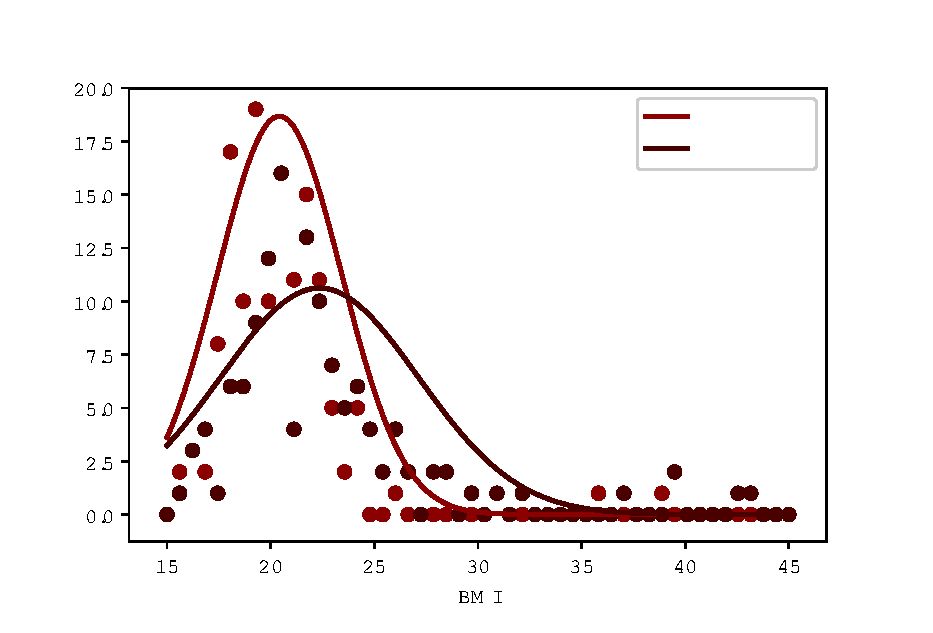
\includegraphics[width = 0.8\linewidth]{t0.eps}
	\caption{是否被暗恋与BMI高斯拟合曲线图} % Figure caption
\end{figure}
\subsection{吸引点排名}
在各种爱情故事中,美貌常常是男女主人公必不可少的,但是,在现实生活中,经历过暗恋的人其实明白,性可能占有更大的成分。为了观测美貌与性格哪一个更为重要,我们来看性格、才艺、美貌在暗恋中的吸引点排第一的比例,如图\ref{c6}。
\begin{figure}[htbp]
	\centering
	\label{c6}
	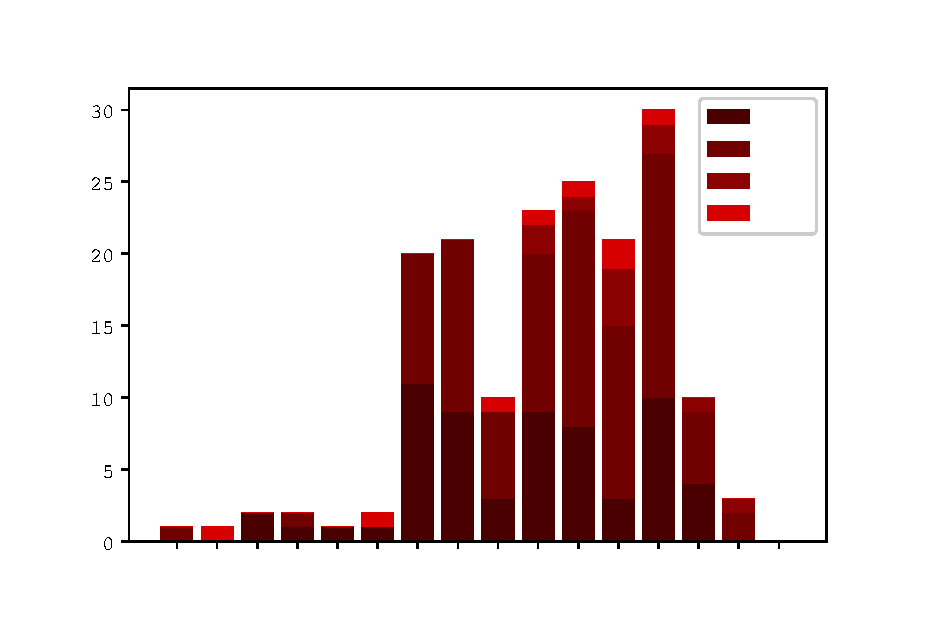
\includegraphics[width = 0.8\linewidth]{c6.eps}
	\caption{第一吸引点与暗恋开始时间统计图} % Figure caption
\end{figure}

从图中可以看到,虽然外貌的占比不小,但是占最大部分的其实是性格。\\
其实,用从认识到开始暗恋的时间跨度可以将暗恋可以分为两类:一类是快速的,也即一见钟情;另一种,是在日常之中缓慢地产生情愫。显然,前一种主要是以对方地外貌为吸引点;而后者,则是以对方的性格作为吸引点。第一种,主要是对方开始便给自己留下了美好的印象,外貌就显得尤其重要,当然,也不排除性格的因素。而第二种,其实更多是在日常生活中逐渐被对方的闪光点吸引,性格便占据了主导地位。\\
\indent 从数据分析来看,在学生时代,其实这两种都是有的,但是,从认识到开始暗恋普遍是存在一定时间跨度的。学生之间往往有更多的相处时间,特别是中学时代,这样学生彼此更能看清对方的性格。假如一个人的外貌美丽,但是性格却使自己无法忍受,那么,那最开始那美貌带给自己的好感也会消失,这样的暗恋便不了了之。而纵使在最开始的时候对方的外貌并没有给自己留下深刻的印象,在以后的日常生活中,对方的行为性格却时时感动自己,那么就很容易对对方产生暗恋心理。\\
\indent 这也从另一个方面对是否被暗恋与BMI的T检验提供了证据:在学生阶段,男女生暗恋的对象择取,重点其实并不在外貌上,健康体现出来的美学自然不会在其中起到大作用,产生不相关的结果也就使正常的了。\\
\indent 我们再来看这三者的排名得分与暗恋开始时间的相关性,由于这两个变量都是线性的,我们采取了线性相关性检验,结果如下:美貌得分的r值为0.200,性格得分的r值为-0.055,才艺得分的r值为-0.114。
这结果是令我们感到惊奇的,美貌的得分与开始时间是呈正相关的,而后两者都与开始时间呈负相关,尽管相关性并不是特别强,但在一定程度上却也可以说明某些问题:随着人的成长,美貌在暗恋中的成分不断上升,而性格与 才艺的地位则是下降的,这一点其实是跟进化心理学吻合的呢。随着年龄越来越靠近为自己将来的人生投资的阶段,人们潜意识那择偶的一面便愈发明显。因此,与健康美学相关的美貌便逐渐得到重视,而与亲代投资并无太大关系的才艺被冷落得也比较快。\\
\subsection{性别与暗恋开始时间}
生理学上,女性的青春期是早于男性的,那么从心理学的角度上看,我们来探测暗恋开始时间与性别的关系。由于开始时间具有线性的性质,我们仍然采用T检验,h0是无相关性,显著性指数为0.05,结果:P=0.428813889,-P=0.428>0.05,说明两者存在很显著的相关性,结果应该算是不出所料的。在青春期,人们的心理会得到快速地成长,因此,女性的心理比男性成熟得早,相应的,女性开始暗恋的时间也就早于男性。\\\\
\subsection{开始时间与从暗恋到告白的间隔时间}
这个的相关性是出乎我们意料的,分析恐怕会有不到位之处,还请谅解。由于这两个均存在线性性质,我们采取了线性相关检验,结果r值为-0.625。
\indent -0.625的r值说明它们之间存在强负相关性,也即随着开始时间的推迟,人们从开始暗恋到告白的间隔时间在逐渐缩小。以下是个人分析所得到的几个可能的原因:\\
\indent 生理上,在青春期的阶段,年龄越大,生理上的成熟就越多一分。而生理上的成熟其实会带给我们一种对异性相处的渴望,这样也就越发能引起我们的告白冲动。\\
心理上,年龄越小,我们的心智就离成熟就越远,因此,其实我们对自己的感情就越不明了,也就越不敢确定是否真的要去告白。而告白成功后的可能的生活也需要一定的心智去接受,因此,心智越成熟的人,对于告白的内心准备也就越充分。\\
\indent 另一个可能的原因,其实来自外部因素,是升学带来的分离。从数据分析可以看出,每一次的升学,都是一次大型的告白现场。因为,人们总是会找各种原因来推迟告白的进行。但是,升学后的分离却能带给他们压力,促使他们去告白。而小学升初中,初中升高中,高中升大学,都是一次可能的分离,但是分离的规模却不尽相同。严格来说,越往后,分离的距离越大,也就越有可能再也见不到对方,因此,它带给暗恋方的压力也就越大,促使暗恋方去告白的效果也就更强。\\
\begin{figure}[htbp]
	\centering
	\label{l0}
	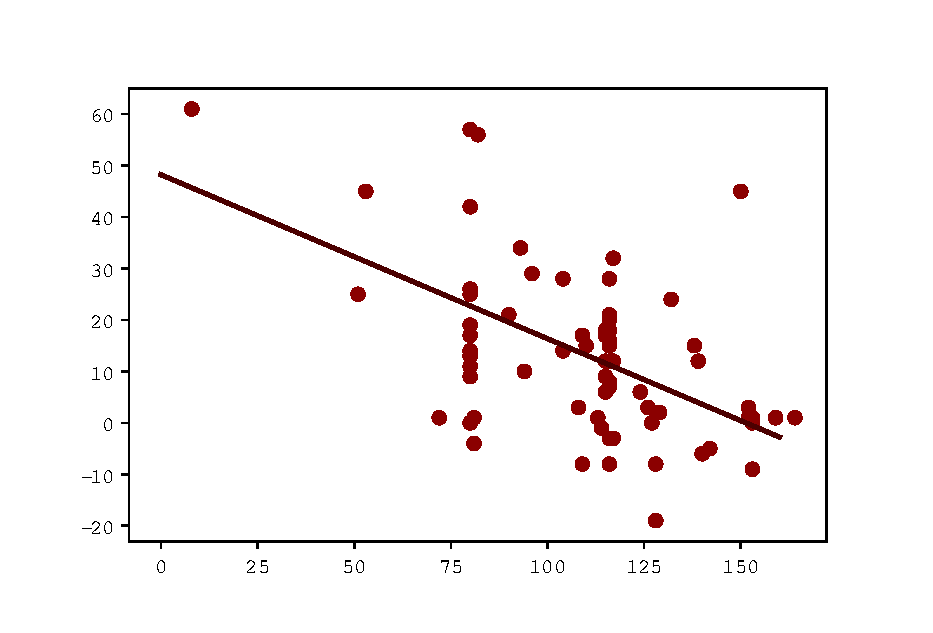
\includegraphics[width = 0.8\linewidth]{l0.eps}
	\caption{开始时间与从暗恋到告白的间隔时间统计图} % Figure caption
\end{figure}
\\
\section{讨论与展望}
总体来说,本文通过统计学的方法得到以下结论,对于高中生来说,他们很容易在自己萌发对某人的爱慕之情之前,就已经不由自主地表现出自己内心的相反。而且,几乎不存在所谓的僚机或助攻,大部分朋友都只会添乱。此外,女生普遍比男生在感情方面先开窍,且女生喜欢的男生种类具有比较强的指向性,而男生们开窍相对较晚,且喜欢的女生类型非常多样。\\
\indent 表达内心想法是一件非常困难的事情,在有过暗恋经历的调查样本中,只有不到四成的人向对方明确表达过自己的态度,有人信心十足却吃了闭门羹,而也有人没多大把握但还是鼓起勇气表达自己的想法,并最终脱单。综合考虑上不做某件事情更容易带来长期后悔,所以我们推荐各位单身人士勇敢地说明自己内心的想法。\\
\indent 当然,我们的调查还有许多诸如样本年龄太过相近,学科太过集中等不足,还有许多可以改进与进一步挖掘的地方。我们所使用的数据与算法均已上传至我们的github页面:https://github.com/richsoap/
pku\_psychology\_2018\_teamwork。\\
%----------------------------------------------------------------------------------------
%	BIBLIOGRAPHY
%----------------------------------------------------------------------------------------
%\bibliographystyle{abbrv}
%\printbibliography[title={参考文献}] % Print the bibliography, section title in curly brackets
%\bibliographystyle{plain}%
%\bibliography{example.bib}
%----------------------------------------------------------------------------------------
\end{document}
